\documentclass{beamer}
\usepackage[CJKspace,space,CJKspace=true]{xeCJK}
\usepackage{fontspec,xunicode}
\setCJKsansfont{PingFang TC}
\setsansfont{Helvetica}
%\setCJKsansfont{Apple LiGothic}
%\setCJKsansfont{Lucida Grande}
\usepackage{xltxtra}
\defaultfontfeatures{Ligatures=TeX}
\usepackage[american]{babel}
\usepackage{setspace}
\usepackage{color}
\usepackage{hyperref}
\usepackage{ruby}
\usepackage{graphics}
\hypersetup{
    colorlinks=true,
    linkbordercolor = {white},
}
\usepackage{listings}
\usepackage{adjustbox}
\defaultfontfeatures{Mapping=tex-text}

\setbeamertemplate{caption}[numbered]
\setbeamertemplate{bibliography item}{\insertbiblabel}

\mode<presentation>

\begin{document}

\title{Exploring Thermal Related Stuff in iDevices using Open-Source Tools \\
  \ruby{Iōng}{用}\ open-source \ruby{kang-k\=u }{工具} \ruby{lâi }{來} \ruby{thàm-khàn }{探看} \ruby{tsáu }{走} iOS ê \ruby{mih-â }{物仔} \ruby{lāi-té }{內底} \ruby{kah }{佮} \ruby{un-tōo }{溫度} \ruby{siong-kuan }{相關} \^e software \ruby{kah }{佮} hardware}

\author[freedom]{T\^an Koan-S\^in \\ \href{mailto:freedom@computer.org}{freedom@computer.org} \\ COSCUP 2019 Lâi Tâi Káng}
\date{December 21, 2019}

\begin{frame}
  \titlepage
\end{frame}

\begin{frame}[allowframebreaks,fragile]
  \frametitle{Table of contents}
  \tableofcontents
\end{frame}

\section{Introduction}
\begin{frame}
  \frametitle{Who am I?}
  \begin{itemize}
  \item ``\ruby{Guá-sī }{我是}  \ruby{tsi̍t-ê }{一个} \ruby{siá }{寫} code \ruby{ê }{个} \ruby{lâng}{人}, \ruby{guá-ê-khóo }{我个苦} \ruby{lóng}{攏} \ruby{siá-tī }{寫佇} \ruby{bīn-tíng}{面頂}'' -- Somebody I Don't Know His Name, COSCUP 2017
  \item Learnt to use open source on a VAX-11/780 running 4.3BSD, before the term ``open source'' was coined
  \item Learnt a bit Pe̍h-ōe-jī about the same time
  \item feel free to interrupt me anytime
  \end{itemize}
\end{frame}

\begin{frame}
  \frametitle{Why this topic?}
  \begin{itemize}
  \item This is the era of so-called ``dark silicon'' \cite{Esmaeilzadeh:2011:DSE:2000064.2000108}.
  \item Thermal control is an important but seldom-talked topic. I could not find public information on how iOS does it.
  \item Recent \href{https://github.com/axi0mX/ipwndfu}{checkm8} \cite{checkm8} and follow-on \href{https://checkra.in/}{checkra1n} \cite{checkra1n} enable jailbreaking of iPhone 5s – iPhone X, iOS 12.3 and up.
  \end{itemize}
\end{frame}

\section{A Peek into Thermal Sensors}
\begin{frame}[allowframebreaks]
  \frametitle{iPhone 6 Thermal Sensors}
  \begin{figure}
    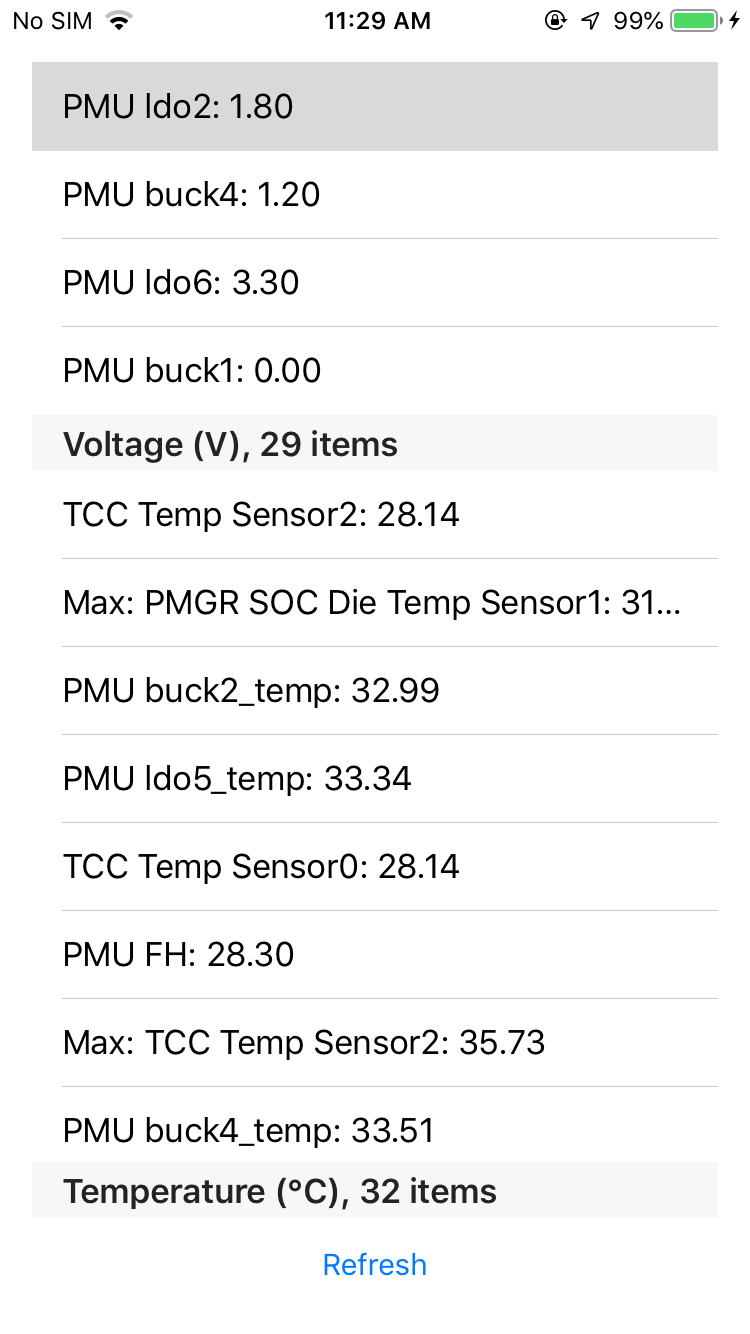
\includegraphics[width=.3\textwidth,keepaspectratio]{iphone6_temp_1.png}
    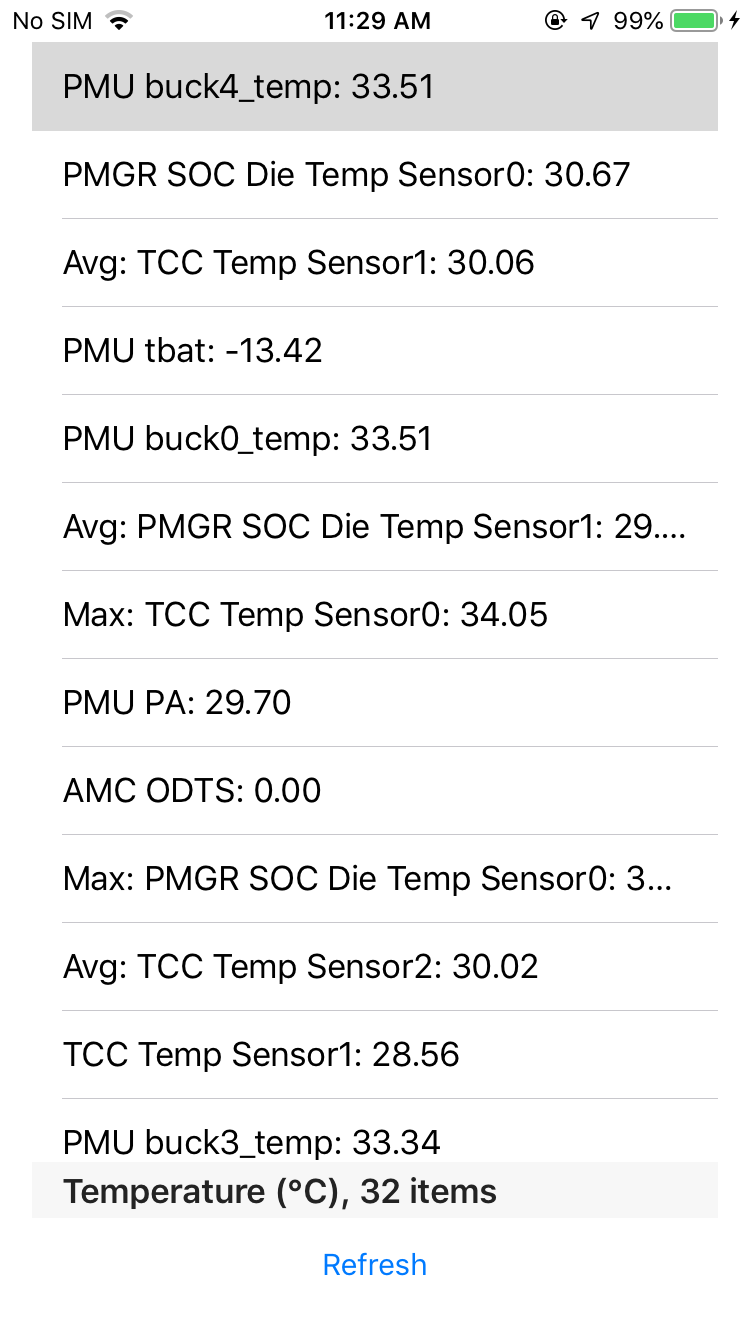
\includegraphics[width=.3\textwidth,keepaspectratio]{iphone6_temp_2.png}
    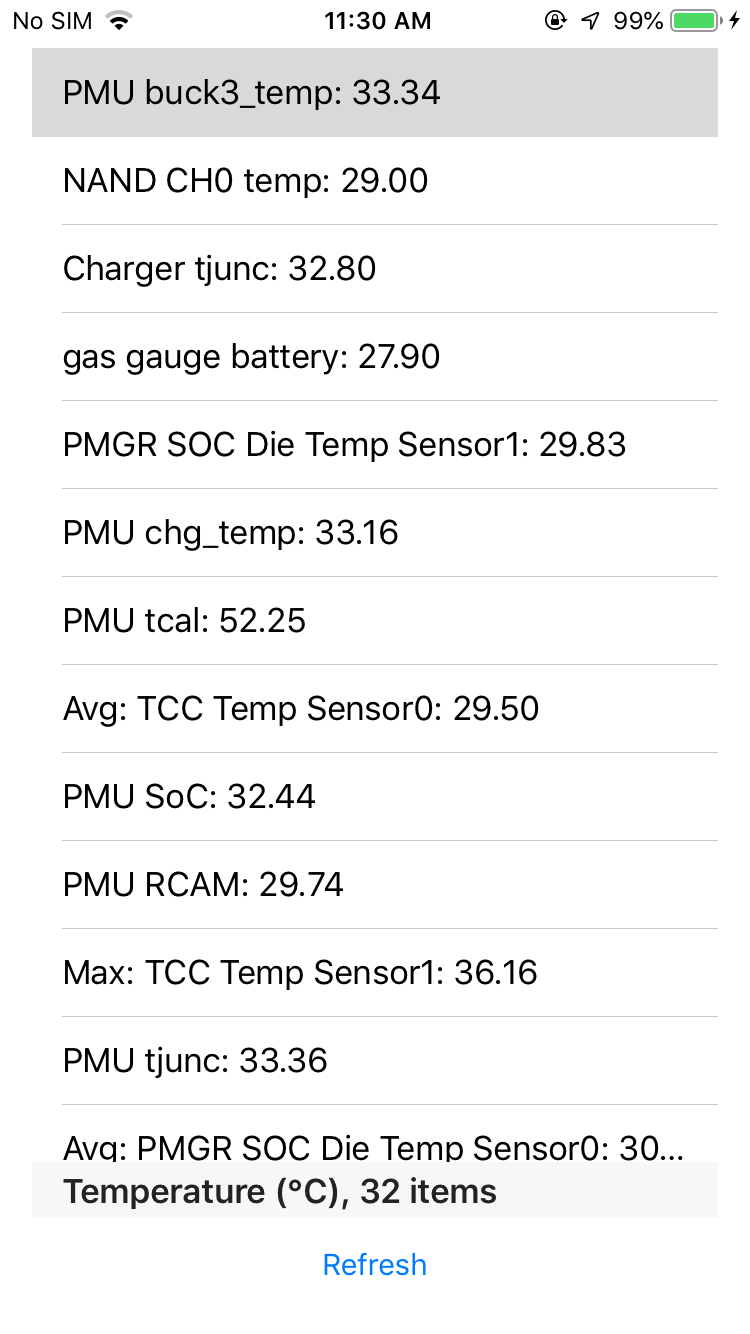
\includegraphics[width=.3\textwidth,keepaspectratio]{iphone6_temp_3.png}
  \end{figure}
  \begin{itemize}
  \item There are 32 thermal sensors (and 21 current and voltage sensors) on iPhone 6!
  \item Above information are from my little program on github \cite{mysensors}.
  \item No jailbreak required, but ``undocumented'' API is used. So don't submit it to App Store (mostly it will be rejected).
  \end{itemize}
\end{frame}

\begin{frame}
  \frametitle{some numbers of sensors}
  \begin{table}
    \begin{tabular}{|| l | r |  r | r||} 
      \hline
      Model & thermal & current & voltage \\
      \hline\hline
      iPhone 6	& 32 & 21 & 29 \\
      \hline
      iPhone 6s & 48 & 27 & 23 \\
      \hline
      iPhone 7 & 47 & 32 & 35 \\
      \hline
      iPhone 8 plus & 68 & 3 & 7 \\
      \hline
      iPhone Xs Max & 67 & 4 & 8 \\
      \hline
      iPhone 11 Pro & 76 & 2 & 6 \\
      \hline
    \end{tabular}
    \caption{Some numbers of sensors I collected}
  \end{table}
\end{frame}

\begin{frame}
  \frametitle{How Does the App Work?}
  \begin{itemize}
  \item IOKit: public and documented on macOS, but not on iOS.
  \item IOKit: Apple ``hidclass''
  \item Code:
    \begin{itemize}
    \item Objective-C: Get sensor information using the IOKit framework
    \item Swift: wrapper. 'Cause I wanna learn a bit Swift.
    \end{itemize}
  \end{itemize}
\end{frame}

\begin{frame}
  \frametitle{IOKit}
  \begin{itemize}
  \item derived from NeXTSTEP's DriverKit, which uses Objective-C \cite{driverkit}. As you might know, in WWDC 2019, the name DriverKit is back in macOS \cite{appledriverkit}.
  \item macOS/iOS device driver development framework: For kernel model divers and user model access \cite{iokit}
    \begin{figure}
      \includegraphics[width=.3\textwidth,keepaspectratio]{iokit-overview.png}
      \caption{Figure from \cite{Singh:2006:MOX:1076423}}
    \end{figure}
  \end{itemize}
\end{frame}

\begin{frame}[fragile,allowframebreaks]
  \frametitle{IOKit HIDClass}
  \begin{itemize}
  \item IOKit/IOKit Family/HID class \cite{iokit:family}: Originally it's for USB, but it's far beyond that now. So there is \textbf{Usage Page}.
  \item a command line tool that can be used to enumrate IOKit devices is \texttt{ioreg(8)}
  \item you can see in Listing \ref{ioreg-output}, there are \texttt{"PrimaryUsage" = 5}, \texttt{"PrimaryUsagePage" = 65280}, and \texttt{"DeviceUsagePairs" = ({"DeviceUsagePage"=65280,"DeviceUsage"=5})}
  \end{itemize}
  
  \begin{adjustbox}{varwidth=\maxdimen,max width=\linewidth,keepaspectratio}
    \begin{lstlisting}[caption={Example TemperatureSensor in \texttt{ioreg} output}, label={ioreg-output}]
    ...
    +-o AppleEmbeddedNVMeTemperatureSensor  <class AppleEmbeddedNVMeTemperatureSensor, id 0x1000003f8, registered, matched, active, busy 0 (1 ms), retain 8>
    | |   |         | | {
    | |   |         | |   "IOCFPlugInTypes" = {"7DDEECA8-A7B4-11DA-8A0E-0014519758EF"="IOHIDFamily.kext/PlugIns/IOHIDLib.plugin","FA12FA38-6F1A-11D4-BA0C-0005028F18D5"="IOHIDFamily.kext/PlugIns/IOHIDLib.plugin"}
    | |   |         | |   "VendorID" = 0
    | |   |         | |   "CountryCode" = 0
    | |   |         | |   "IOUserClientClass" = "IOHIDEventServiceUserClient"
    | |   |         | |   "Product" = "NAND CH0 temp"
    | |   |         | |   "VersionNumber" = 0
    | |   |         | |   "IOGeneralInterest" = "IOCommand is not serializable"
    | |   |         | |   "PrimaryUsage" = 5
    | |   |         | |   "LocationID" = 1414410350
    | |   |         | |   "HIDEventServiceProperties" = {"DeviceOpenedByEventSystem"=Yes,"PreserveTimestamp"=Yes,"BatchInterval"=1,"LogLevel"=6}
    | |   |         | |   "ProductID" = 0
    | |   |         | |   "DeviceUsagePairs" = ({"DeviceUsagePage"=65280,"DeviceUsage"=5})
    | |   |         | |   "Built-In" = Yes
    | |   |         | |   "ReportInterval" = 0
    | |   |         | |   "HIDServiceSupport" = Yes
    | |   |         | |   "PrimaryUsagePage" = 65280
    | |   |         | |   "VendorIDSource" = 0
    | |   |         | |   "QueueSize" = 0
    | |   |         | | }
    ...
    \end{lstlisting}
  \end{adjustbox}

\end{frame}

\begin{frame}
  \frametitle{Build the App}
  \begin{itemize}
  \item if you \texttt{git clone} the source code and try to build it, you will get error message saying IOKit related header can't be found (of course, you know you have to change signing stuff)
  \item you have to borrow them from macOS SDK,
    \begin{enumerate}
    \item \texttt{pushd .}
    \item \texttt{cd \path{/Applications/Xcode.app/Contents/Developer/Platforms/iPhoneOS.platform/Developer/SDKs/iPhoneOS.sdk/System/Library/Frameworks/IOKit.framework/}}
    \item \texttt{sudo ln -s \path{/Applications/Xcode.app/Contents/Developer/Platforms/MacOSX.platform/Developer/SDKs/MacOSX.sdk/System/Library/Frameworks/IOKit.framework/Headers} .}
    \item \texttt{popd}
    \end{enumerate}
  \end{itemize}
\end{frame}

\begin{frame}
  \frametitle{The devil is in the detail}
  \begin{itemize}
  \item some non public data types
    \begin{itemize}
    \item \href{https://opensource.apple.com/source/IOHIDFamily/IOHIDFamily-701.60.2/IOHIDFamily/AppleHIDUsageTables.h.auto.html}{AppleHIDUsageTables}
    \item \href{https://opensource.apple.com/source/IOHIDFamily/IOHIDFamily-701.60.2/IOHIDFamily/IOHIDEventTypes.h.auto.html}{IOHIDEventTypes}
    \end{itemize}
    \item some functions from source code. e.g., \texttt{IOHIDEventSystemClientRef IOHIDEventSystemClientCreate(CFAllocatorRef allocator);}
  \end{itemize}
\end{frame}

\section{More Thermal Control Related Mechanisms}
\begin{frame}[allowframebreaks]
  \frametitle{More Thermal Control Related Mechanisms}
  \begin{itemize}
  \item There is \path{/usr/libexec/thermalmonitord} in iOS 13 (\path{/usr/libexec/mobilewatchdog} in iOS 12.x), which collects thermal information and does thermal-throttling when necessary.
  \item The thermalmonitord is mainly written in Objective-C (how to know that? there are Objective-C sections in Mach-O).
  \item Mach-O has been around for more than 30 years.There are many tools we can used to inspect Mach-O files. E.g., if you know binutils, llvm-based binutils.
  \item \texttt{class-dump}, one of the interesting Mach-O tools, could extract Objective-C class related information (including protocols and methods) from Mach-O files and convert those them to Objective-C headers.
    \begin{itemize}
    \item \texttt{class-dump thermalmonitord} of iPhone 8 running iOS 13.3 (\texttt{class-dump thermalmonitord -H -o /tmp/thermal\_headers}), we can get more than 100 headers.
    \end{itemize}
  \item How about runtime infomation? So far, I think \texttt{cycript} \cite{cycript} is the most convenient tool if you are willing to learn a new language.
  \end{itemize}
\end{frame}

\begin{frame}
  \begin{figure}
    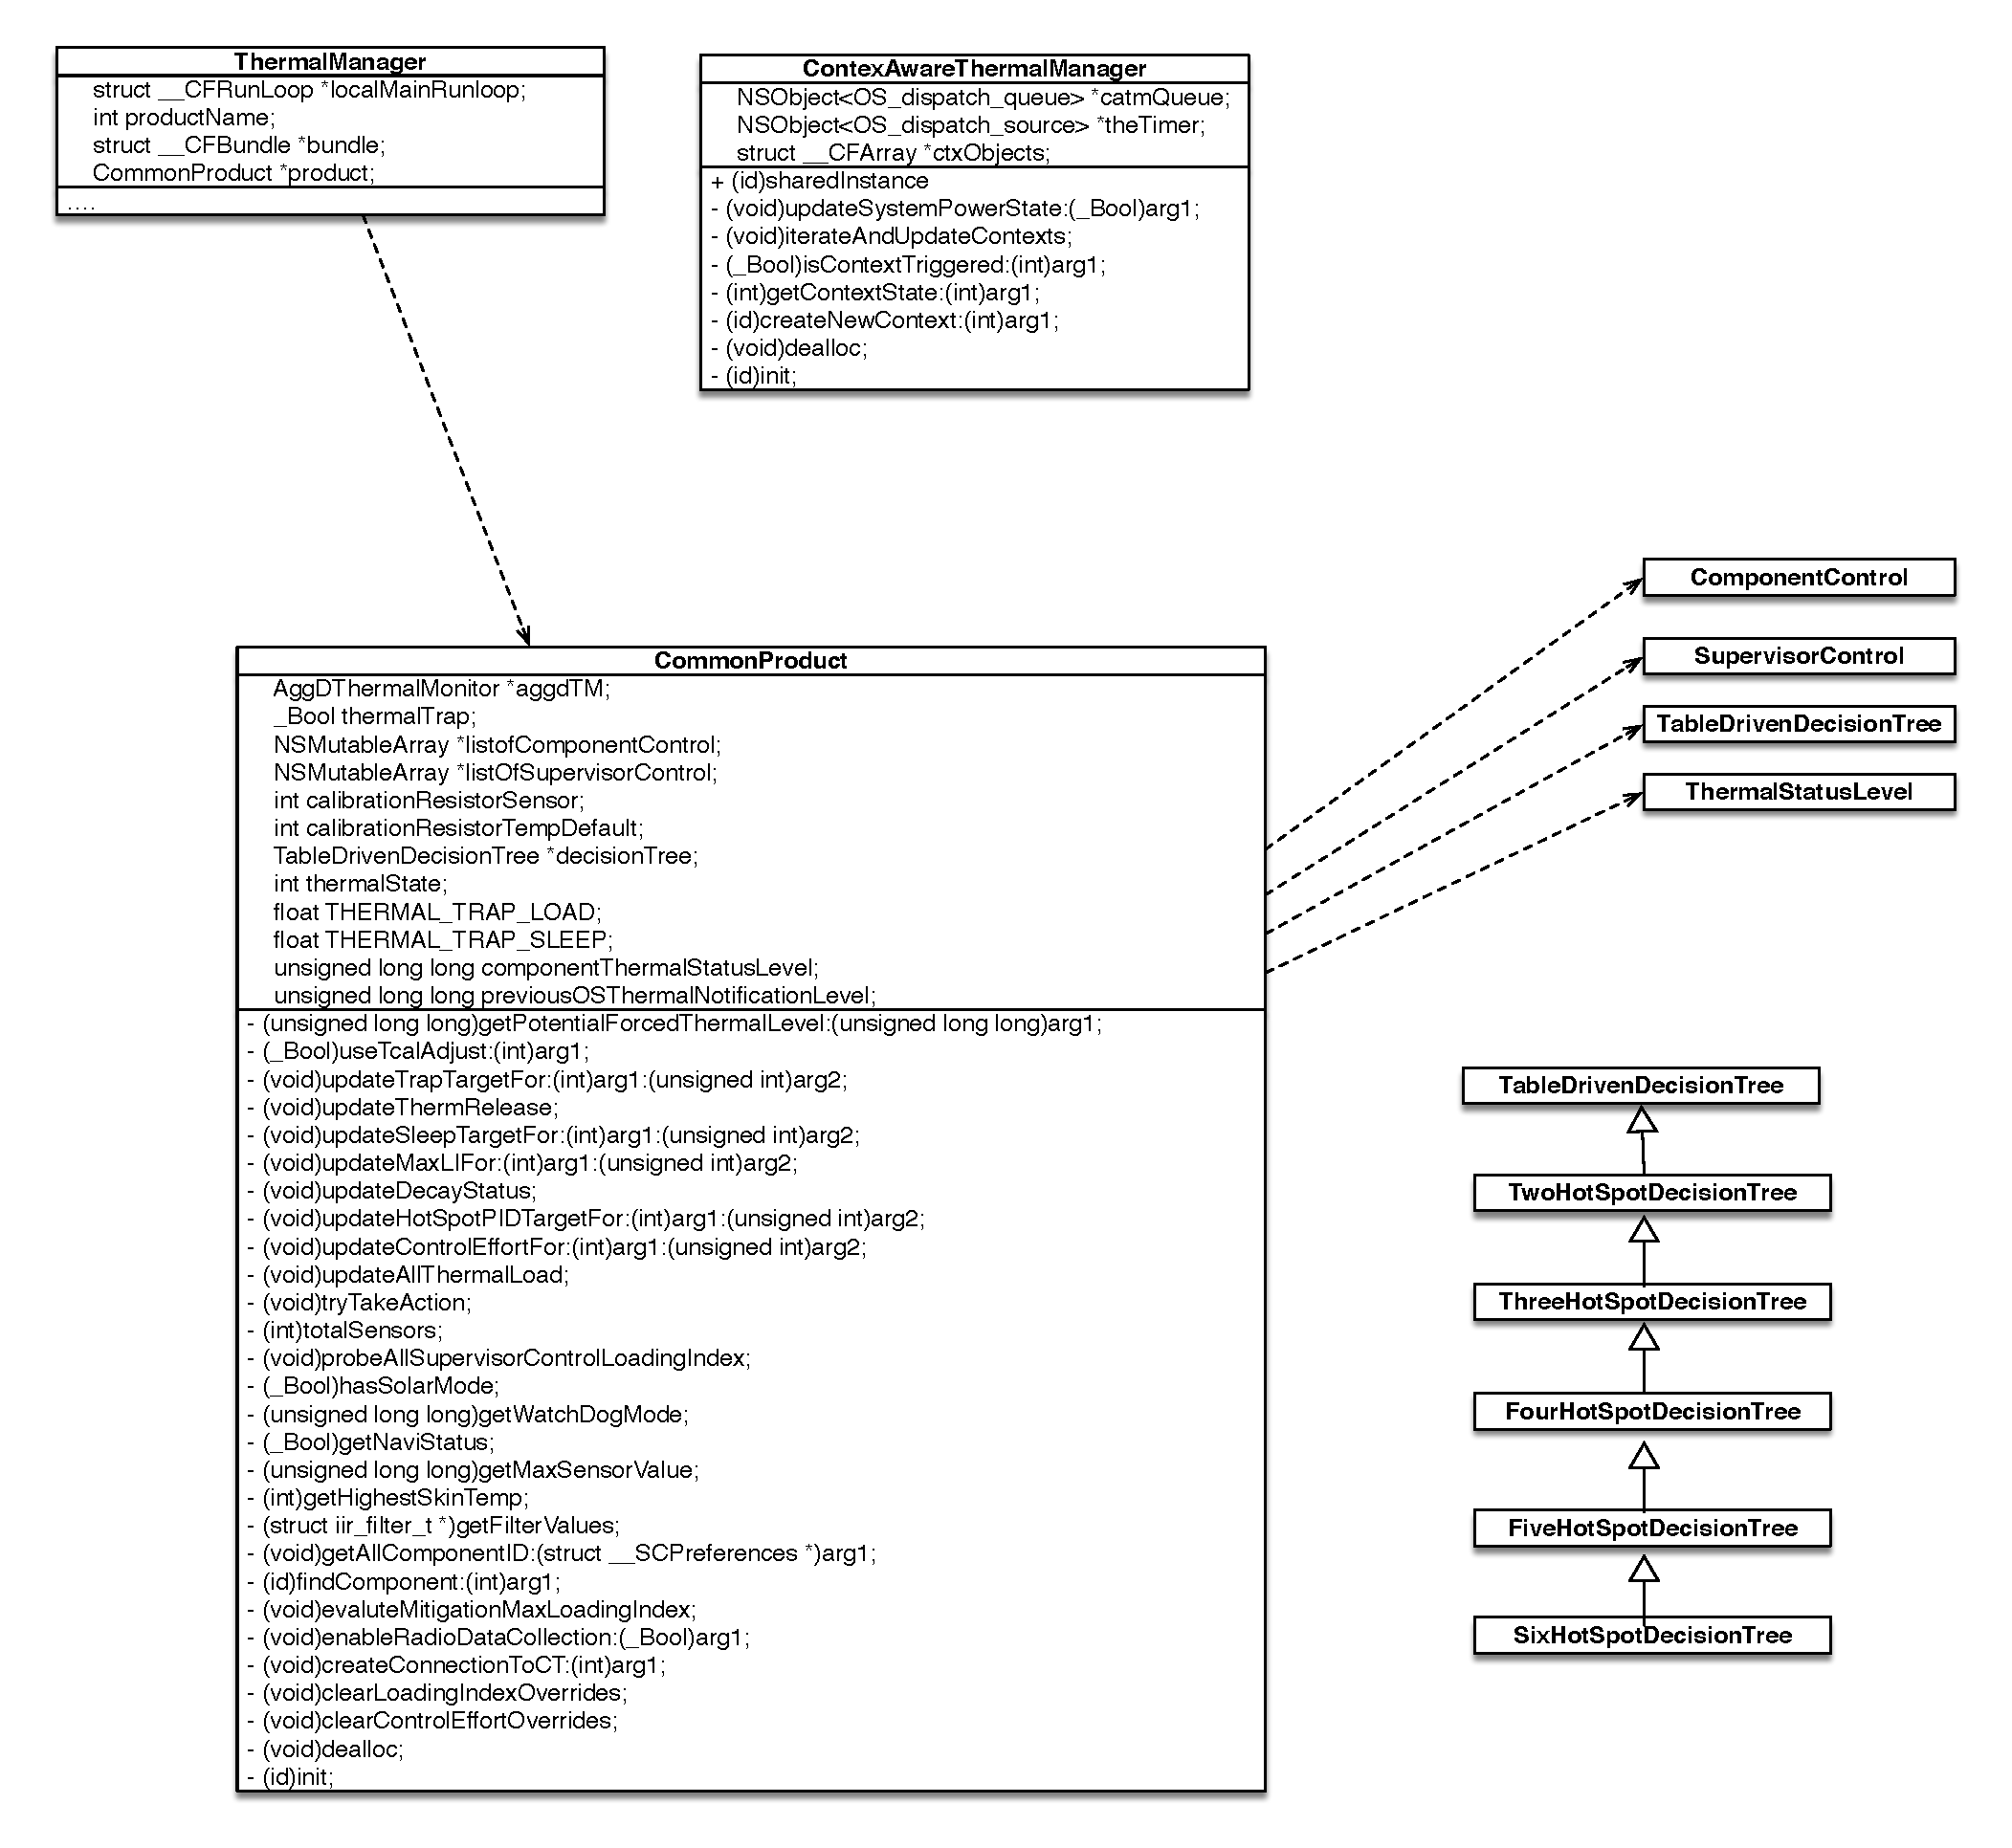
\includegraphics[height=.8\textheight,keepaspectratio]{ios-thermal-manager.pdf}
    \caption{iOS Thermal Manager}
  \end{figure}
\end{frame}

\begin{frame}
  \begin{figure}
    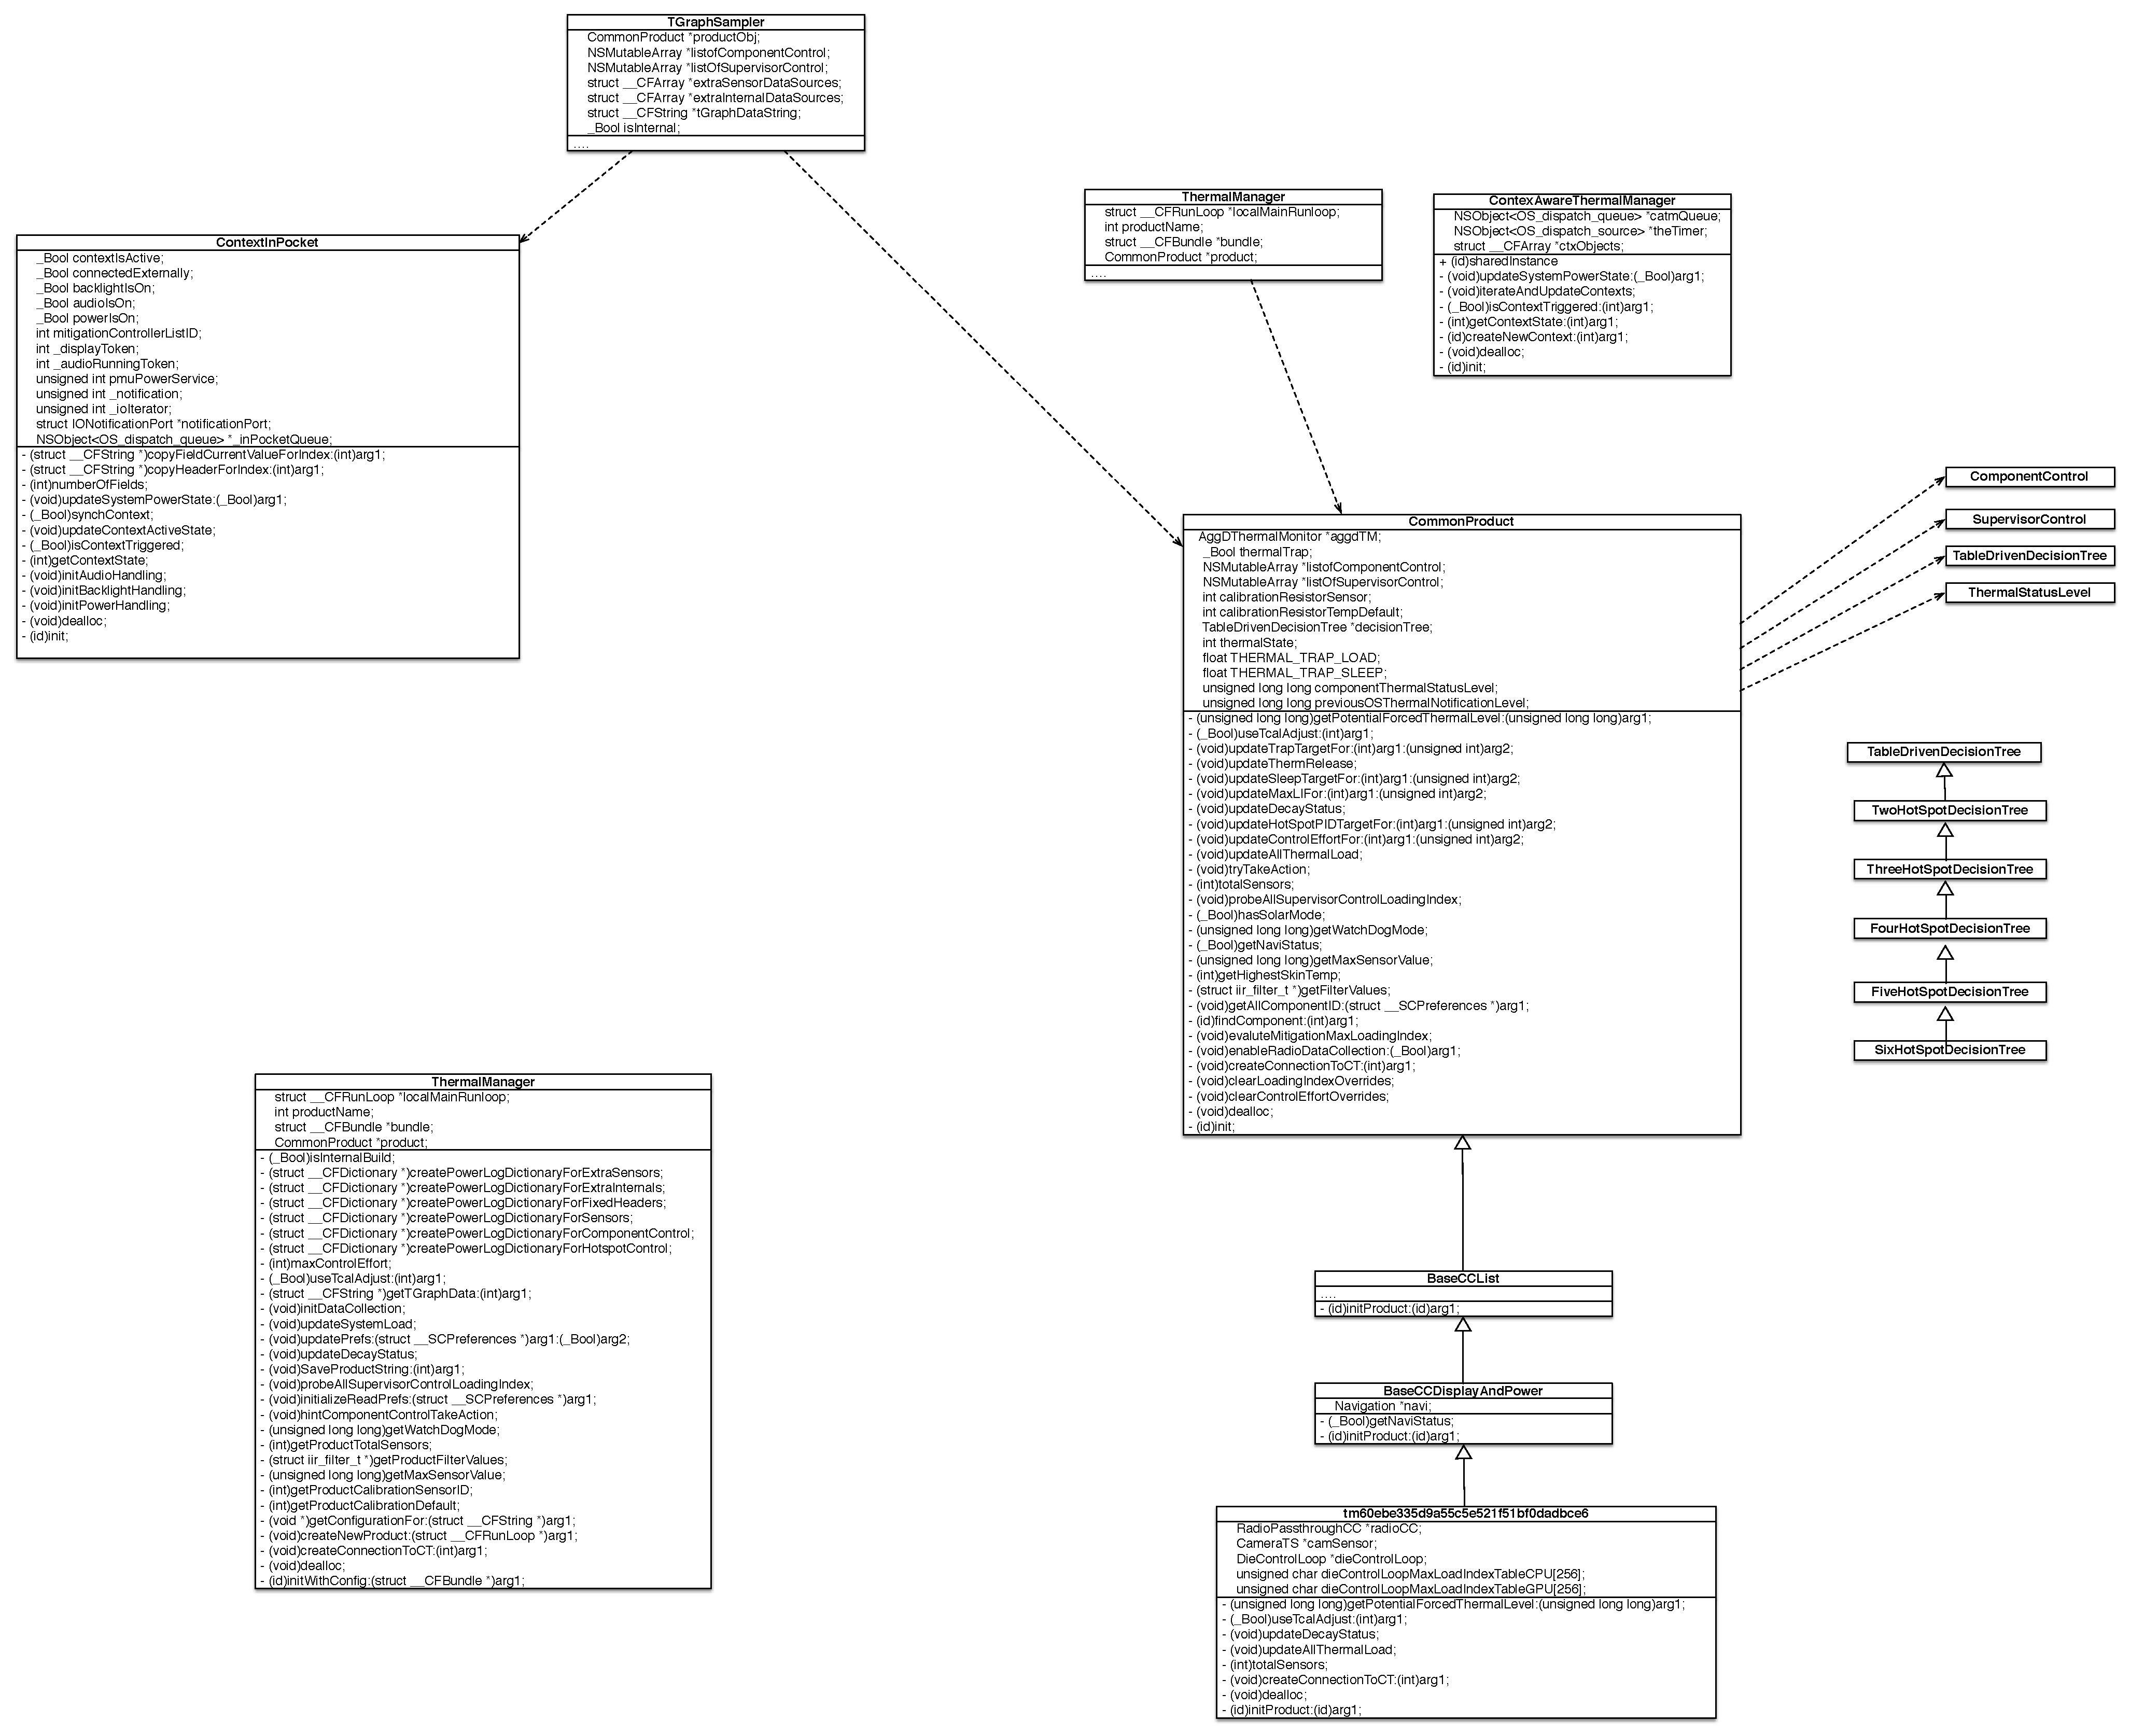
\includegraphics[height=.8\textheight,keepaspectratio]{ios-thermal-manager-more.pdf}
    \caption{iOS Thermal Manager and others}
  \end{figure}
\end{frame}

\begin{frame}
  \begin{figure}
    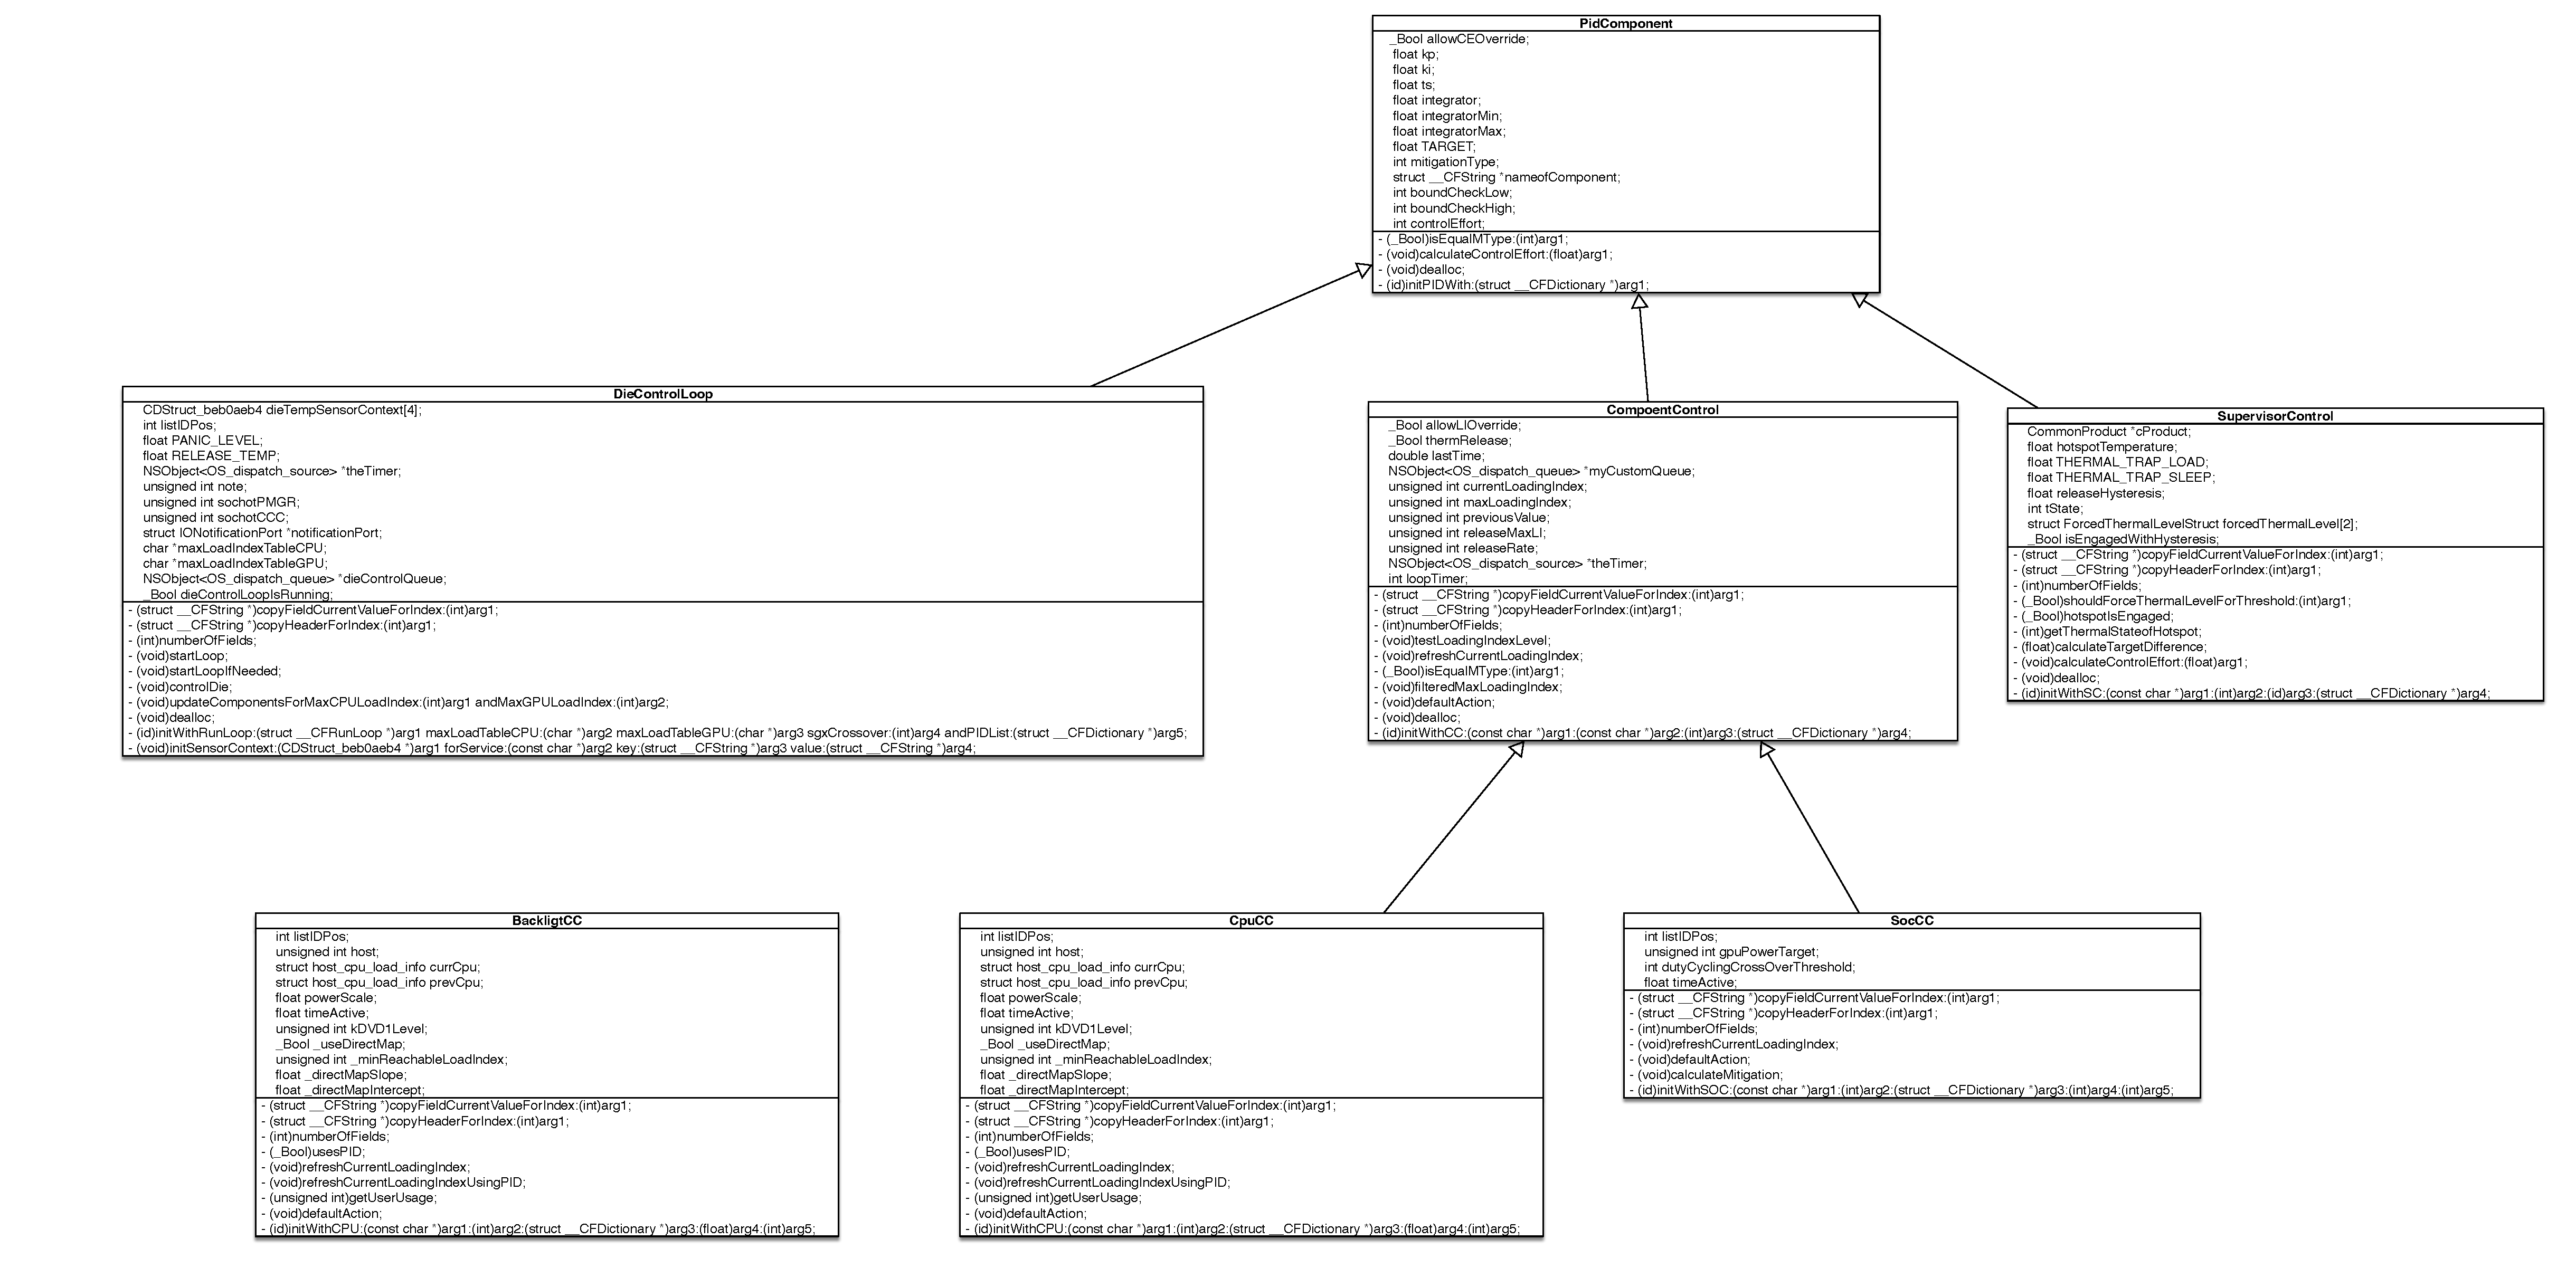
\includegraphics[width=.8\textwidth,keepaspectratio]{iOS-thermal.pdf}
    \caption{Example iOS Thermal Control Loops}
  \end{figure}
\end{frame}

\begin{frame}
  \frametitle{Yes, PID control is used}
  \begin{figure}
    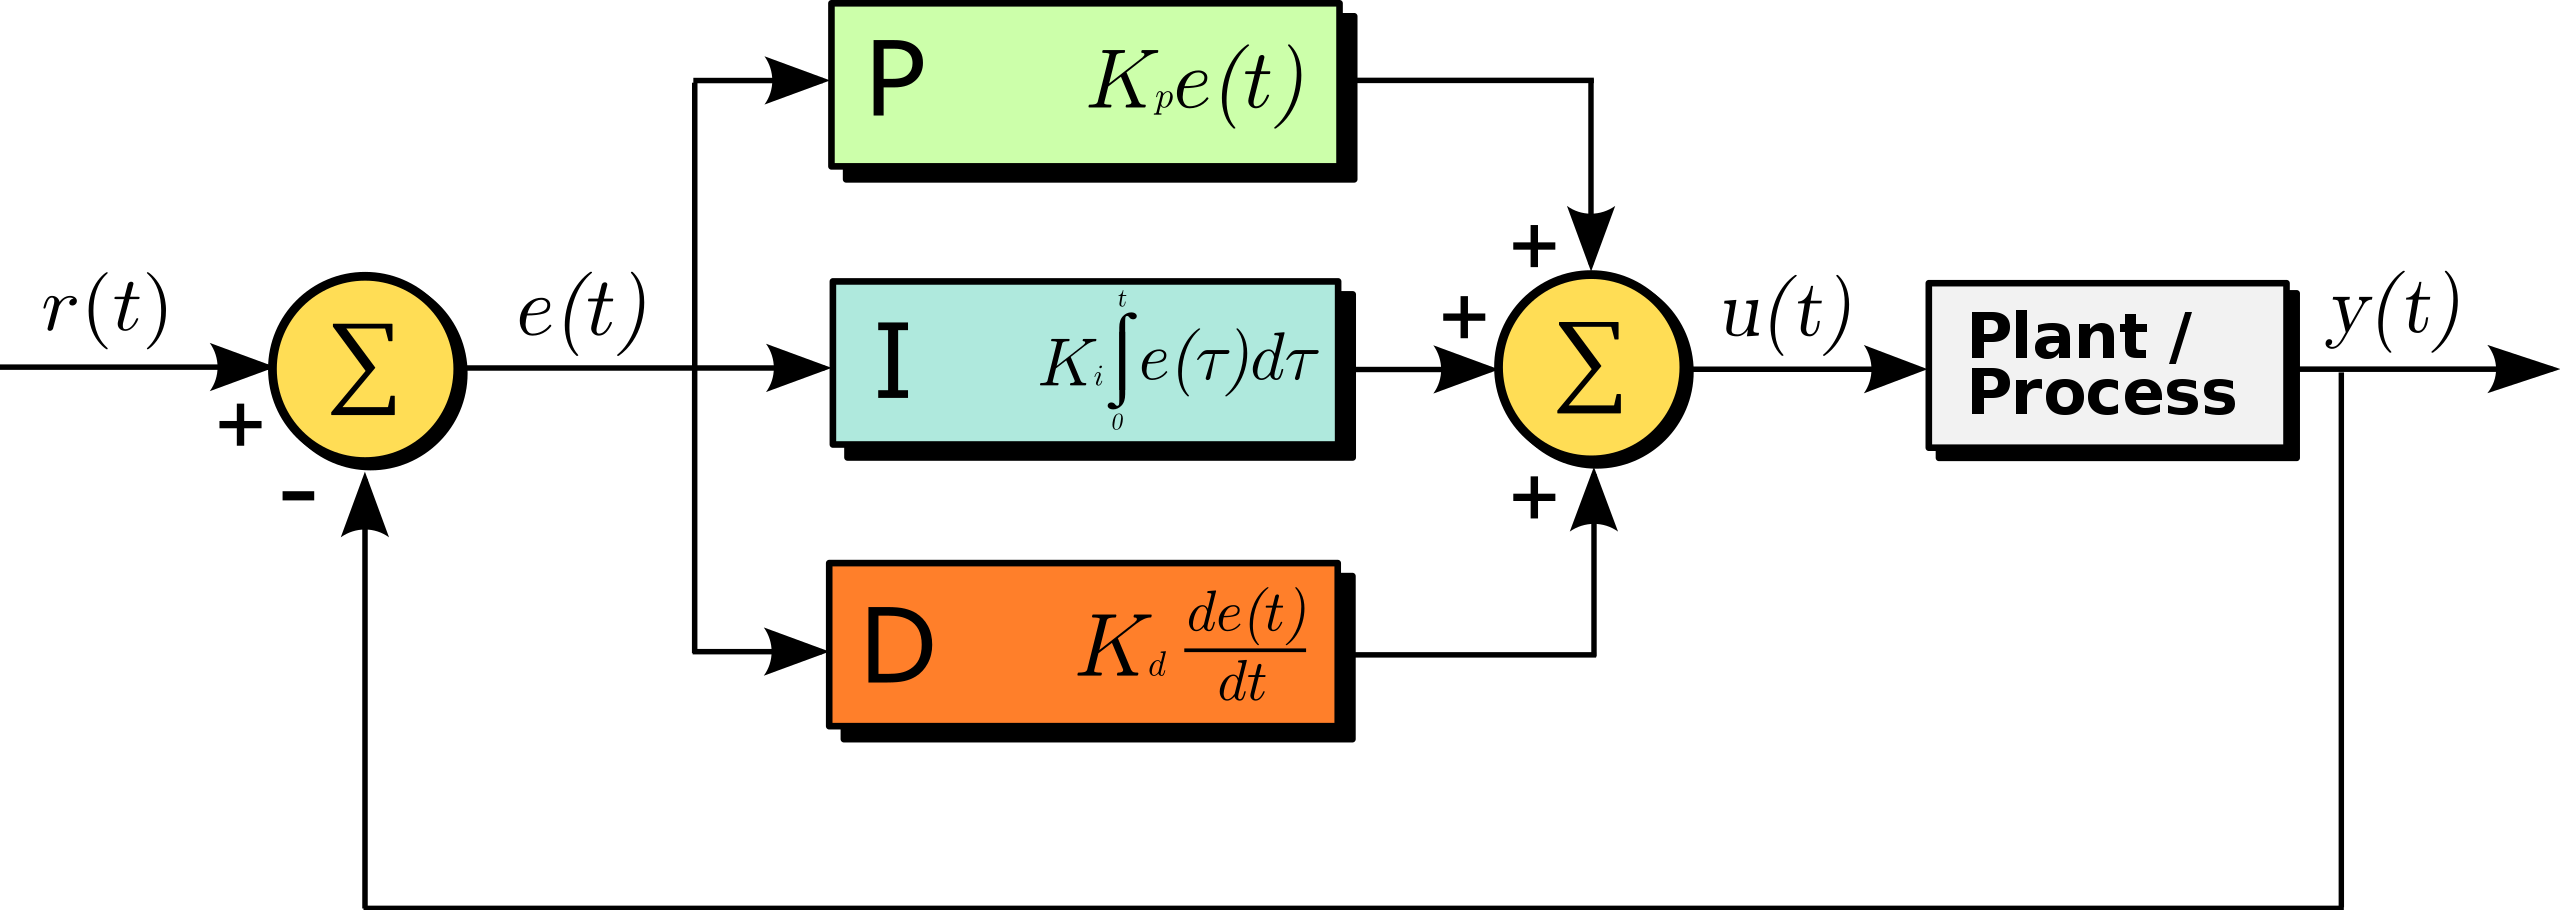
\includegraphics[width=.8\textwidth,keepaspectratio]{PID_en.png}
    \caption{PID figure from Wikipedia, \url{https://en.wikipedia.org/wiki/PID_controller}}
  \end{figure}
\end{frame}

\begin{frame}[allowframebreaks,fragile]
  \frametitle{peeking running systems with cycript}
  \begin{itemize}
  \item attaching cycript to a running system process is a bit more complicated after iOS 12. We could start from a wrapper called cycrun, \url{https://www.reddit.com/r/jailbreakdevelopers/comments/b1r5kq/question\_is\_cycript\_coming\_to\_ios\_12\_unc0ver\_jb/}
  \item with \texttt{cyrun+cycript},
  \item \texttt{cyrun -x thermalmonitord -e}
  \item then where to start, singleton ones are less intrusive and easier
  \item as you see, we can get \texttt{productObj}
  \item as you can see, the \texttt{thermalmonitord} uses HID sensors.
  \end{itemize}

  \tiny
  \begin{adjustbox}{varwidth=\maxdimen,max width=\linewidth,keepaspectratio}
    \begin{lstlisting}[basicstyle=\tiny,caption={Cyrun},label=cyrun,breaklines]
~ root# cyrun -x thermalmonitord -e 
applicationName: thermalmonitord is running (64)
    executableName: thermalmonitord
    bundleIdentifier: 
    Cycript is active: thermalmonitord
    Device is passcode locked
    Tweak Mode
Success, Cycript was already active for the Process. You may now run
    cycript -r 127.0.0.1:8556
cy# tgs = [TGraphSampler sharedInstance]
#"<TGraphSampler: 0x104f04330>"
cy# tgs->productObj 
#"<tm0148f449e0ff00c77f11492610c521ce: 0x104f04090>"
cy# tgs->
__defineGetter__                              extratGraphDataSources
__defineSetter__                              gotDataToLogToLiteMode
__lookupGetter__                              hasOwnProperty
__lookupSetter__                              isInternal
__proto__                                     isPrototypeOf
_appleCareState                               isa
_appleCareStateLastLogged                     lastLogTimestamp
_powerlogQueue                                listOfSupervisorControl
_powerlogSubkeyController_Components          listofComponentControl
_powerlogSubkeyController_HiP                 previousThermalSensorValues
_powerlogSubkeyController_Hotspots            productObj
_powerlogSubkeyController_LiteMode            propertyIsEnumerable
_powerlogSubkeyController_MiscExternalState   tGraphDataString
_powerlogSubkeyController_MiscInternalState   toLocaleString
_powerlogSubkeyController_Sensors             toString
_powerlogSubkeyController_Sensors_Components  valueOf
constructor
    \end{lstlisting}
  \end{adjustbox}

  \begin{adjustbox}{varwidth=\maxdimen,max width=\linewidth,keepaspectratio}
    \begin{lstlisting}[basicstyle=\tiny,caption={Cycript HidSensos},label=cycript-hidsensors,breaklines]
cy# hs =  [HidSensors sharedInstance]
#"<HidSensors: 0x10582bac0>"
cy# new Instance(hs->_tempSensors)[0]
#"+++++++++++++++++++++++++++++++++++++++++++++++++++++++++++++++++++++++++++\n
RegistryID:          0x0000000100000277\n
BuiltIn:             1\n
Product:             Avg: PMGR SOC Die Temp Sensor0\n
LocationID:          1416114273\n
VendorID:            0\n
ProductID:           0\n
CountryCode:         0\n
PrimaryUsagePage:    65280\n
PrimaryUsage:        5\n
DeviceUsagePairs:   \n
    DeviceUsagePage:     65280\n
    DeviceUsage:         5\n
+++++++++++++++++++++++++++++++++++++++++++++++++++++++++++++++++++++++++++\n"
cy# 
    \end{lstlisting}
  \end{adjustbox}
\end{frame}

\section{Other Tools}
\begin{frame}[allowframebreaks,fragile]
  \frametitle{Other tools}
  \begin{itemize}
  \item binutils and other hacking tools, such as lsof
  \item lldb/gdb on devices: Apple used to ship ``fat'' gdb and lldb, but not anymore(?). LLDB allows using Objective-C style syntax (most iOS programmers before Swift was introduced know Objective-C).
  \item remote debbuging: either cross building or native building of lldb could be an ostacle, if you are not afraind of using remote debugging, they (debuggserver and lldb) are open source too. Example usage (my iMAC: \texttt{192.168.1.80}, the iPhone: \texttt{192.168.1.115)}
    \begin{enumerate}
    \item install \texttt{debuggerserver} on your iDevice. Then, run \texttt{debugserver 192.168.1.80:5555 --attach=thermalmonitord} to wait for connection from \texttt{192.168.1.80} to port 5555 of this devices.
    \item on you host, launch \texttt{lldb}, then use \texttt{platform select remote-ios} and \texttt{process connect connect://192.168.1.115:5555} to connect to the \texttt{debugserver} on the remote device. You should see something like Listing ~\ref{connect-to-lldb}
    \item we can examine \texttt{TGraphSampler} as in Listing ~\ref{TGraphSampler}
    \item and \texttt{HidSenors} as in Listing ~\ref{HidSensors}
    \end{enumerate}
    \item \textbf{NOTE: DON'T interrupt the \texttt{thermalmonitord} too long, otherwise the device will reboot.}
  \end{itemize}
  
  \tiny  
  \begin{lstlisting}[basicstyle=\tiny,caption={connect to debugserver from lldb},label={connect-to-lldb}]
(lldb) platform select remote-ios
  Platform: remote-ios
 Connected: no
  SDK Path: "/Users/freedom/Library/Developer/Xcode/iOS DeviceSupport/13.3 (17C54)"
 SDK Roots: [ 0] "/Users/freedom/Library/Developer/Xcode/iOS DeviceSupport/13.3 (17C54)"
(lldb) process connect connect://192.168.1.115:5555
Process 64 stopped
* thread #1, queue = 'com.apple.main-thread', stop reason = signal SIGSTOP
    frame #0: 0x0000000184864634 libsystem_kernel.dylib`mach_msg_trap + 8
libsystem_kernel.dylib`mach_msg_trap:
->  0x184864634 <+8>: ret    

libsystem_kernel.dylib`mach_msg_overwrite_trap:
    0x184864638 <+0>: mov    x16, #-0x20
    0x18486463c <+4>: svc    #0x80
    0x184864640 <+8>: ret    
Target 0: (thermalmonitord) stopped.
  \end{lstlisting}
  
  \begin{lstlisting}[basicstyle=\tiny,caption={TGraphSampler},label=TGraphSampler]
(lldb) expr TGraphSampler* $tgs = [TGraphSampler sharedInstance]
(lldb) p *$tgs
(TGraphSampler) $0 = {
  NSObject = {
    isa = TGraphSampler
  }
  productObj = 0x0000000103e03f80
  listofComponentControl = 0x0000000103e041a0 @"9 elements"
  listOfSupervisorControl = 0x0000000103e041d0 @"12 elements"
  extratGraphDataSources = 0x0000000103e04520
  tGraphDataString = 0x0000000000000000
  isInternal = false
  gotDataToLogToLiteMode = false
  lastLogTimestamp = 38967673125
  previousThermalSensorValues = {
    [0] = 0
    [1] = 0
    [2] = 0
    [3] = 0
    [4] = 0
    [5] = 0
    [6] = 0
    [7] = 0
    [8] = 0
    [9] = 0
    [10] = 0
    [11] = 0
    [12] = 0
    [13] = 0
    [14] = 0
    [15] = 0
    [16] = 0
    [17] = 0
    [18] = 0
    [19] = 0
    [20] = 0
    [21] = 0
    [22] = 0
    [23] = 0
    [24] = 0
    [25] = 0
    [26] = 0
    [27] = 0
    [28] = 0
    [29] = 0
    [30] = 0
    [31] = 0
    [32] = 0
    [33] = 0
    [34] = 0
    [35] = 0
    [36] = 0
    [37] = 0
    [38] = 0
    [39] = 0
    [40] = 0
    [41] = 0
    [42] = 0
    [43] = 0
    [44] = 0
    [45] = 0
    [46] = 0
    [47] = 0
    [48] = 0
    [49] = 0
    [50] = 0
    [51] = 0
    [52] = 0
    [53] = 0
    [54] = 0
    [55] = 0
    [56] = 0
    [57] = 0
    [58] = 0
    [59] = 0
    [60] = 0
    [61] = 0
    [62] = 0
    [63] = 0
  }
  _powerlogQueue = 0x0000000103e04850
  _powerlogSubkeyController_Hotspots = 0x0000000103e04610
  _powerlogSubkeyController_Components = 0x0000000103e04690
  _powerlogSubkeyController_Sensors = 0x0000000103e046d0
  _powerlogSubkeyController_MiscInternalState = 0x0000000103e04710
  _powerlogSubkeyController_MiscExternalState = 0x0000000103e04750
  _powerlogSubkeyController_LiteMode = 0x0000000103e04790
  _powerlogSubkeyController_HiP = 0x0000000103e047d0
  _powerlogSubkeyController_Sensors_Components = 0x0000000103e04810
  _appleCareState = 0x0000000103e048d0 @"5 elements"
  _appleCareStateLastLogged = 0x0000000103e04af0 @"5 elements"
 }
(lldb) po $tgs->productObj
<tm0148f449e0ff00c77f11492610c521ce: 0x103e03f80>    
    \end{lstlisting}
  %\end{adjustbox}
  
  \begin{lstlisting}[basicstyle=\tiny,caption=''HidSensors'',label=HidSensors]
(lldb) expr HidSensors * $hs = [HidSensors sharedInstance]
(lldb) p *$hs
(HidSensors) $1 = {
  NSObject = {
    isa = HidSensors
  }
  _hidEventSystem = 0x0000000103d0f9c0
  _infoOnlyHIDSensors = 0x0000000103f2d400
  _callbackSensorIntervals = 0x0000000103f2cc10
  _readFailuresExpected = 0x0000000000000000
  _powerSensors = 0x0000000000000000
  hidSensorKeys = 0x0000000103e037a0
  sensorFourCharCode = 0x0000000103e03db0
  synthSensorKeys = 0x0000000103e03de0
  _callbackTemperatures = 0x0000000103f31630
  _potentiallyStaleSensorTimestamps = 0x0000000103e03e10
  _potentiallyStaleSensorDefaults = 0x0000000103f2c840
  _callbackTemperaturesQueue = 0x0000000103f2d570
  sensorWatchdogMask = 1236950581247
  _infoOnlySensorsActive = false
  _dispatchVirtualTemp = true
  _send2DTempGrid = false
  _tempSensors = 0x0000000105015fc0
  _count = 36
  _shadowSensorCount = 8
  _sensorDict = 0x0000000103f30e80
  _serviceToName = 0x0000000103f31670
}
(lldb) po $hs->_tempSensors
<__NSArrayI 0x105015fc0>(
+++++++++++++++++++++++++++++++++++++++++++++++++++++++++++++++++++++++++++
RegistryID:          0x0000000100000270
BuiltIn:             1
Product:             Max: PMGR SOC Die Temp Sensor3
LocationID:          1416115064
VendorID:            0
ProductID:           0
CountryCode:         0
PrimaryUsagePage:    65280
PrimaryUsage:        5
DeviceUsagePairs:   
    DeviceUsagePage:     65280
    DeviceUsage:         5
+++++++++++++++++++++++++++++++++++++++++++++++++++++++++++++++++++++++++++
,
....    
  \end{lstlisting}
\end{frame}

\begin{frame}
  \frametitle{concluding remarks}
  \begin{itemize}
  \item iOS uses many open source components and you can use open source tools to explore iDevices.
  \item how about Android devices: as far as I can tell, most Android devices the ``standard'' Linux thermal framework.
  \end{itemize}
\end{frame}

\begin{frame}[allowframebreaks,fragile]
  \frametitle{References}
  \tiny
  \bibliography{ref}
  \bibliographystyle{acm}
\end{frame}

\end{document}
